%%%%%%%%%%%%%%%%%%%%%%%%%%%%%%%%%%%%%%%%%
% Journal Article
% LaTeX Template
% Version 1.4 (15/5/16)
%
% This template has been downloaded from:
% http://www.LaTeXTemplates.com
%
% Original author:
% Frits Wenneker (http://www.howtotex.com) with extensive modifications by
% Vel (vel@LaTeXTemplates.com)
%
% License:
% CC BY-NC-SA 3.0 (http://creativecommons.org/licenses/by-nc-sa/3.0/)
%
%%%%%%%%%%%%%%%%%%%%%%%%%%%%%%%%%%%%%%%%%

%----------------------------------------------------------------------------------------
%	PACKAGES AND OTHER DOCUMENT CONFIGURATIONS
%----------------------------------------------------------------------------------------

\documentclass[twoside,twocolumn]{article}

\usepackage{blindtext} % Package to generate dummy text throughout this template

\usepackage[sc]{mathpazo} % Use the Palatino font
\usepackage[T1]{fontenc} % Use 8-bit encoding that has 256 glyphs
\linespread{1.05} % Line spacing - Palatino needs more space between lines
\usepackage{microtype} % Slightly tweak font spacing for aesthetics

\usepackage[english]{babel} % Language hyphenation and typographical rules
\usepackage{graphicx}

\usepackage[hmarginratio=1:1,top=32mm,columnsep=20pt]{geometry} % Document margins
\usepackage[hang, small,labelfont=bf,up,textfont=it,up]{caption} % Custom captions under/above floats in tables or figures
\usepackage{booktabs} % Horizontal rules in tables

\usepackage{lettrine} % The lettrine is the first enlarged letter at the beginning of the text
\usepackage{algorithm}
\usepackage[noend]{algpseudocode}
\usepackage{amsmath}

\usepackage{enumitem} % Customized lists
\setlist[itemize]{noitemsep} % Make itemize lists more compact

\usepackage{abstract} % Allows abstract customization
\renewcommand{\abstractnamefont}{\normalfont\bfseries} % Set the "Abstract" text to bold
\renewcommand{\abstracttextfont}{\normalfont\small\itshape} % Set the abstract itself to small italic text

\usepackage{titlesec} % Allows customization of titles
\renewcommand\thesection{\Roman{section}} % Roman numerals for the sections
\renewcommand\thesubsection{\roman{subsection}} % roman numerals for subsections
\titleformat{\section}[block]{\large\scshape\centering}{\thesection.}{1em}{} % Change the look of the section titles
\titleformat{\subsection}[block]{\large}{\thesubsection.}{1em}{} % Change the look of the section titles

\usepackage{fancyhdr} % Headers and footers
\pagestyle{fancy} % All pages have headers and footers
\fancyhead{} % Blank out the default header
\fancyfoot{} % Blank out the default footer
\fancyhead[C]{Bayesian Optimization in Model Predictive Control $\bullet$ Frederic Dlugi $\bullet$ January 2022} % Custom header text
\fancyfoot[RO,LE]{\thepage} % Custom footer text

\usepackage{titling} % Customizing the title section

\usepackage{hyperref} % For hyperlinks in the PDF

%----------------------------------------------------------------------------------------
%	TITLE SECTION
%----------------------------------------------------------------------------------------

\setlength{\droptitle}{-4\baselineskip} % Move the title up

\pretitle{\begin{center}\Huge\bfseries} % Article title formatting
\posttitle{\end{center}} % Article title closing formatting
\title{Bayesian Optimization in Model Predictive Control} % Article title
\author{%
\textsc{Frederic Dlugi}\\[1ex] % Your name
\normalsize Universität zu Lübeck \\ % Your institution
\normalsize \href{mailto:frederic.dlugi@student.uni-luebeck.de}{frederic.dlugi@student.uni-luebeck.de} % Your email address
%\and % Uncomment if 2 authors are required, duplicate these 4 lines if more
%\textsc{Jane Smith}\thanks{Corresponding author} \\[1ex] % Second author's name
%\normalsize University of Utah \\ % Second author's institution
%\normalsize \href{mailto:jane@smith.com}{jane@smith.com} % Second author's email address
}
\date{\today} % Leave empty to omit a date
\renewcommand{\maketitlehookd}{%
\begin{abstract}
\noindent When using MPC to control a vehicle it is often neccesary to fine tune control and vehicle parameters to get good performance in reality. This is a time consuming process that often relies on trial and error or grid search of the parameter space. In this paper we evaluate the use of Bayesian Optimization to tackle this problem. We simulate vehicle dynamics of a simple bicycle model with two parameters. We try to find the MPC cost ratios and real vehicle parameters by optimizing controller performance with different parameters using Bayesian Optimization.
\end{abstract}
}

%----------------------------------------------------------------------------------------

\begin{document}

% Print the title
\maketitle

%----------------------------------------------------------------------------------------
%	ARTICLE CONTENTS
%----------------------------------------------------------------------------------------

\section{Introduction}

\lettrine[nindent=0em,lines=3]{W} e start by introducing bayesian optimization and MPC on a high level.
This is done to let you know what I understand when talking about these algorithms.

\subsection{What is Bayesian Optimization?}
Bayesian optimization is a strategy for global optimization of backbox functions. (Alg. \ref{alg:bo})
It therefore does not require the computation of gradients, but works best on continuous functions.
It is best suited for optimizing functions, where each evaluation takes a long time.
The number of input dimensions for bayesian optimization is typically less then $20$ \cite{frazier2018tutorial}.
Bayesian Optimization uses an aquisition function that operates on a gaussian process of the evaluations. In this paper we evaluate three different acquisition functions: Expected Improvement (Alg. \ref{alg:ei}), Probability of Improvement (Alg. \ref{alg:poi}) and Upper Confidence Bound (Alg. \ref{alg:ucb}). We use the Matern ($\nu=2.5$) kernel for all experiments. We also vary the $\alpha$ Parameter of the Gaussian Process to smooth out the cost landscape.

\begin{algorithm}
    \caption{Bayesian Optimization}
    \label{alg:bo}
    \begin{algorithmic}
        \State $\text{f} \gets \text{black box function}$
        \State $\text{initPos} \gets \text{initial positions}$
        \State $\text{evaluations} \gets \text{f(initPos)}$
        \For{$i= 1 \to N$}
            \State $\alpha \gets \text{acquisitionFunction(evaluations)}$
            \State $\text{nextPos} \gets \text{argmax(}\alpha\text{)}$
            \State $\text{evaluations}.append(\text{f(nextPos)})$
        \EndFor
        \State $result \gets \text{max(evaluations)}$
    \end{algorithmic}
\end{algorithm}

\begin{algorithm}
    \caption{Expected Improvement}
    \label{alg:ei}
    \begin{algorithmic}
        \State $\mu, \sigma \gets \text{gp.predict(x)}$
        \State $z \gets (\mu - y_{max} - xi)/\sigma$
        \State $result \gets (\mu - y_{max} - xi) * \text{cdf(z)} + \sigma * \text{pdf(z)}$
    \end{algorithmic}
\end{algorithm}

\begin{algorithm}
    \caption{Probability of Improvement}
    \label{alg:poi}
    \begin{algorithmic}
        \State $\mu, \sigma \gets \text{gp.predict(x)}$
        \State $z \gets (\mu - y_{max} - xi)/\sigma$
        \State $result \gets \text{cdf(z)}$
    \end{algorithmic}
\end{algorithm}

\begin{algorithm}
    \caption{Upper Confidence Bound}
    \label{alg:ucb}
    \begin{algorithmic}
        \State $\mu, \sigma \gets \text{gp.predict(x)}$
        \State $result \gets \mu + \kappa * \sigma$
    \end{algorithmic}
\end{algorithm}

\subsection{What is MPC?}
MPC is an acronym for model predicive control.
It replaces classical control algorithms that usually work in an offline manner with an optimizer, that solves the optimal control problem for a receding horizon (Figure \ref{fig:mpc}).
Each action taken is the first action of the optimal control plan.
The plan gets updated continuously (Figure \ref{fig:mpc_plan}), this is called receding horizon approach.

\begin{figure}[h]
    \caption{Blockdiagram of MPC algorithm}
    \centering
    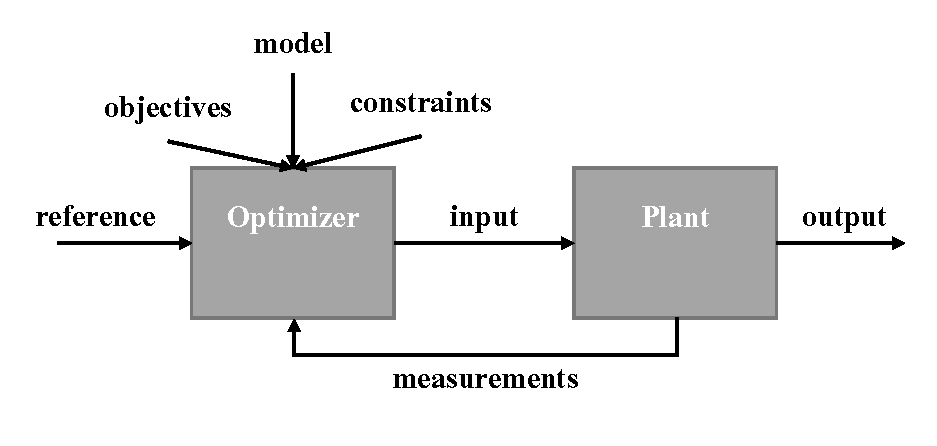
\includegraphics[width=0.45\textwidth]{fig_mpc.pdf}
    \label{fig:mpc}
\end{figure}

\begin{figure}[h]
    \caption{Plan horizon of MPC algorithm}
    \centering
    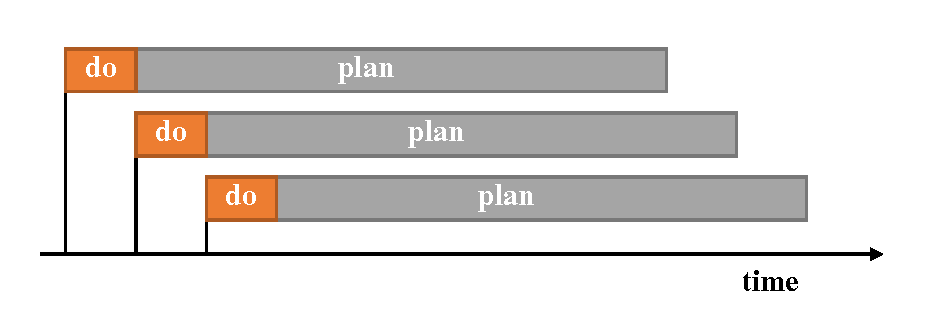
\includegraphics[width=0.45\textwidth]{fig_mpc_plan.pdf}
    \label{fig:mpc_plan}
\end{figure}

\subsection{Kinematic Bicycle Model}

We use a kinematic bicycle model defined by algorithm \ref{alg:kbm} and \ref{alg:ubm} \cite{kinematicBicycleModel}. We try to estimate the $L_r$ and $L_f$ in this paper.
\begin{algorithm}
    \caption{Kinematic Bicycle Model}
    \label{alg:kbm}
    \begin{algorithmic}
        \State $a \gets \text{accelaration (input)}$
        \State $\omega \gets \text{steering angle rate (input)}$
        \State $x_c, y_c \gets \text{center position}$
        \State $v \gets \text{speed}$
        \State $\theta \gets \text{absolute angle}$
        \State $\delta \gets \text{steering angle}$
        \State $\beta \gets \text{side slip factor}$
        \State $L_r \gets \text{Distance center to rear wheel}$
        \State $L_f \gets \text{Distance center to font wheel}$
        \State $L \gets L_r + L_f$
    \end{algorithmic}
\end{algorithm}

\begin{algorithm}
    \caption{Update Bicycle Model}
    \label{alg:ubm}
    \begin{algorithmic}
        \State $\dot{v} \gets a$
        \State $\dot{x_c} \gets v * \cos{(\theta + \beta)}$
        \State $\dot{y_c} \gets v * \sin{(\theta + \beta)}$
        \State $\dot{\theta} \gets v * \cos{(\beta)} * \tan{(\delta)} / L$
        \State $\dot{\delta} \gets \omega$
        \State $\beta \gets \text{atan2}(L_r * \tan{(\delta)}, L)$
    \end{algorithmic}
\end{algorithm}

\section{State of the art}
In Multi-Objective Optimization of a Path-following MPC for Vehicle Guidance \cite{gharib2021multi} BO was used to weight error terms to find the ratio results in the best reference tracking performance of a complex vehicle model in a simulation. Using BO with expected improvement as acquisition function. They found the BO algorithm used to be more efficient then random search when comparing the number of evaluations needed to find satisfactory results.

Lukas Hewing and colaborators \cite{hewing2018cautious} explored the use of BO to decrease model missmatch. They learned a dynamics model of a miniature race car using a gaussian process from real data, while the vehicle is controlled through MPC. They experimented with sparse approximations to gaussian processes to use them in real-time applications.

What papers did similar things?
What where their problems?
What did they achieve?
What do we do differently?

\section{Experiments}

In this paper we explore two uses of BO in the MPC context. First we try to find the optimal ratio between input (accelaration and steering angle rate) cost and reference tracking ($x - x_{ref}$ and $y - y_{ref}$). Secondly we try to find vehicle specific parameters using BO.
\subsection{Experiment setup}
Show specific MPC implementation. Optimizer used is scipys SLSQP.
Show cost function
Show setup with graph
Show generate function
Name number of evaluations per BO step and number of BO steps.

\subsection{Exploring MPC cost ratio using BO}
Compare different acquisition functions.
Cost ratio was explored with different vehicle parameters (show different gaussian processes)

\subsection{Finding Vehicle parameters using BO}
Using different target parameters
Using different acquisition functions
Show main target (1.2, 0.8) -> accumulate all evaluations in one gaussian process

\section{Conclusion}
There is no general ratio between input and reference cost. It depends on vehicle parameters. The optimal ratio is still similar.
Finetuning still required. Using many different reference tracks, leads to better results.

\section{Further research}
Use more suffisticated MPC. Try more hyper parameters. Try if this works on real hardware or using one simple and one complex vehicle model. Try measuring more or less vehicle states. Add uncertency to measurents and model.

\bibliographystyle{plain}
\bibliography{refs.bib}

\end{document}
